\chapter{Electrospray ionization source}
\label{chap:ESI}

\section{Overview of the electrospray and its components}
As the source of molecular ions for the experiment we implement a so-called electrospray ionization (ESI) source \textcolor{red}{FENN,STEEN}. The ESI source we use can be seen connected to the rest of the experiment on \cref{fig:fullSetup}.
\begin{figure}
    \centering
    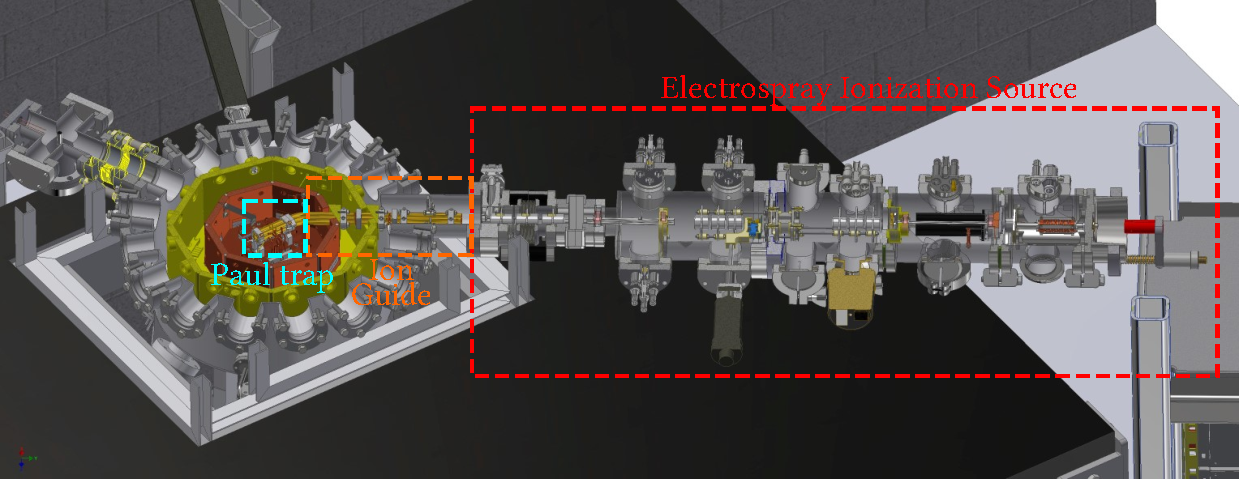
\includegraphics[width = 1.1\textwidth]{main/spray.pdf}
    \caption{3D figure of the full setup at Aarhus, when the electrospray (red) is conneacted to the cryogenic trap. The ion guide (orange) allows to transfer the ions into the cryogenic Paul trap (blue), where experiments will be conducted. At the time of writing the ESI source is not hooked up to the experiment, and instead there is channeltron detector at the very end of the electrospray, where it would connect to the ion guide.}
    \label{fig:fullSetup}
\end{figure}
The basics of how such a device functions is that it has a syringe containg a solvent (typically methanol) with the ions or molecules one wishes to perform experiments on. The syringe is connected to a needle, and a motor slowly depresses the plunger on the syring, causing the solvent to form a droplet on the tip of the needle. The needletip of the ESI source is sitting outside the vaccuum chambers of the ESI setup, in atmospheric air as can be seen on fig..
Opposite of the needle is a narrow opening into the full body of the ESI source, which is put at a very large voltage difference to the tip of the needle (typically 3-3.5kV), this voltage difference leads to a strong electric field which will drag ion droplets from the needle and into the narrow opening of the ionization source.
The ions then enter a capillary tube (see \cref{fig:esiDrawing}) heated to 70 degrees celsius, which is set at some voltage (typically 40V).
\begin{figure}
    \centering
    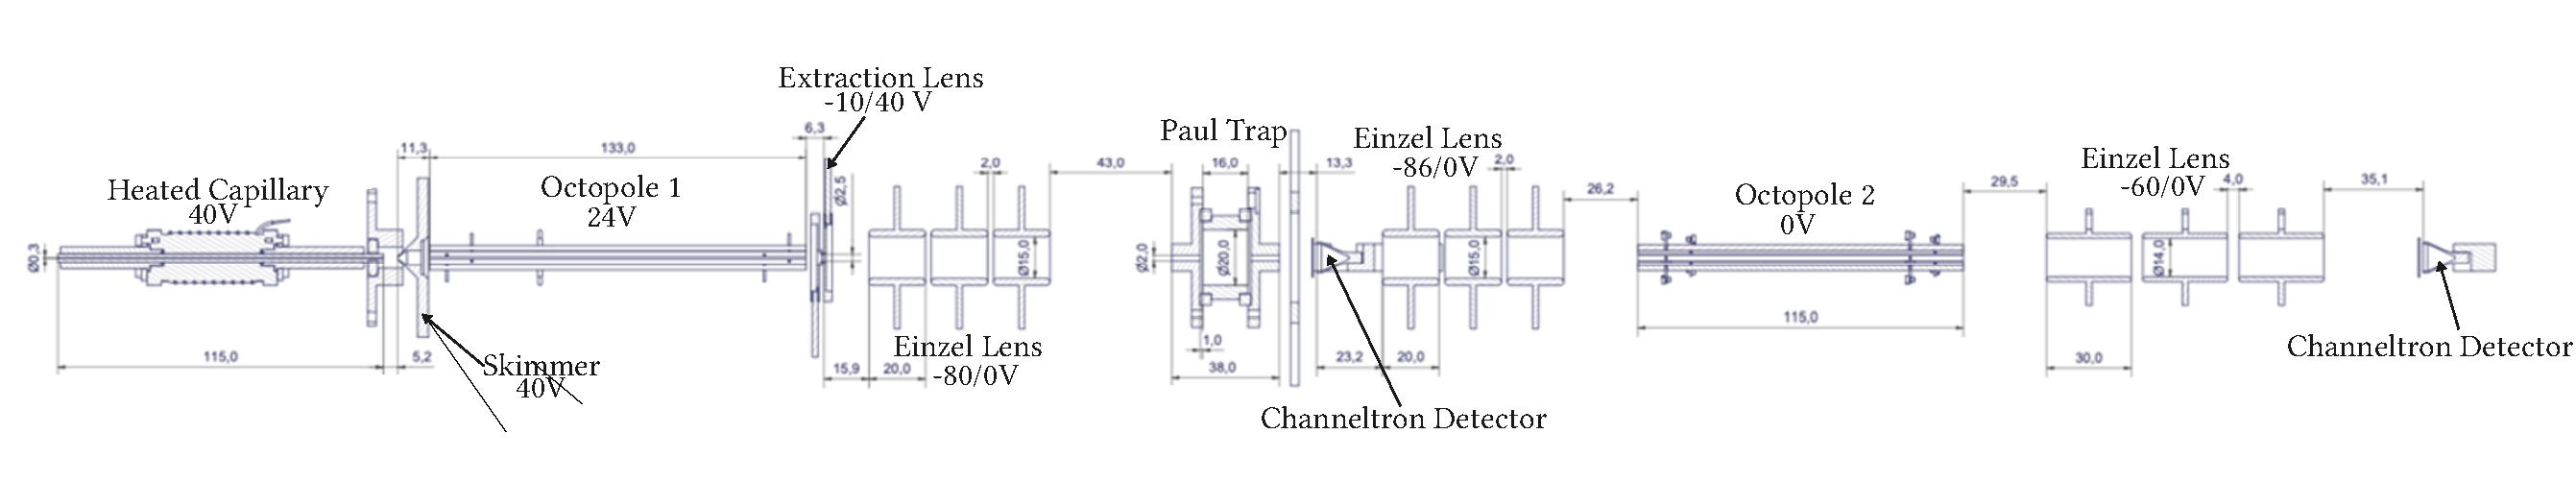
\includegraphics[width = 1.1\textwidth]{main/electrospray_elements.pdf}
    \caption{Technical drawing giving a sideview of all the components of the ESI source we employ. Some of the most important components on the figure have been labelled by name and the voltages typically emplyed on them.
    It is very important to ensure that there is a voltage gradient as one progresses down the ESI source, since otherwise the ions cannot travel. The multiple voltages noted for the Einzel lenses correspond to outer/inner electrode voltages, and for the extraction lens, the low voltage is set for extraction, while the high is for accumulation.}
    \label{fig:esiDrawing}
\end{figure}
Within the heated cappillary the solvent will begin to evaporate, causing the droplets to shrink. This causes the Coulomb repulsion of the ions within the droplet to increase as they all move nearer.
Eventually the surface tension of the droplet can no longer compensate the electrostatic repulsion of the ions within, and the droplet splits. This process repeats until all the solvent is evaporated and the ions are situated in the gas-phase. A schematic of this principle is illustrated on \cref{fig:evaporation}.
\begin{figure}
    \centering
    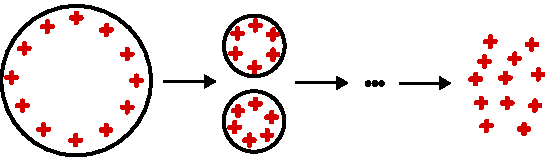
\includegraphics{main/evaporation.pdf}
    \caption{Illustration of the evaporation principle that allows for gas-phase ions in electrospraying. As the solvent evaporates, the droplet will shrink, until the surface tension becomes unable to counteract the electrostatic repulsion of the ions. This splits the droplet into two droplets, for which this process then repeats. Eventually all the solvent is evaporated and only gas-phase ions are left. Note that the number of ions within a droplet has been grossly underestimated for ease of illustration}
    \label{fig:evaporation}
\end{figure}

After the evaporation process, gas-phase ions travel past a skimmer and into an octopole storage device. The octopole allows for efficient transport of the ions across long regions, as well as a source of buffer gas cooling to room temperature, due to ion-neutral collisions with the atmospheric gas at a pressure of approx 1mbar. At the very end of the octopole is a pair of "extraction" lenses. We have timed control of these electrodes, allowing us to set them to bunch electrodes in the octopole by setting a high voltage on them, and then releasing the ion bunch by lowering the voltage. I have performed several experiments on this part of the trap, to characterize the storage capabilities of the octopole, as well as the form of the ion bunches that arrive from it. The results of those investigations are found in \cref{sec:octopoleExperiments}.

Upon extraction from the octopole the ions pass through an Einzel lens. This is a set of three electrodes, where the outer two share the same voltage, and fulfills the same role for ions as a lens does for optics. We use the Einzel lens to focus down the ion beam onto the 2mm wide opening of a cylindrical Paul trap.

The cylindrical Paul trap has two different settings. The first is using it as an Einzel lens, where the front and back electrodes act as the outer electrodes, while the main cylinder acts as the center electrode. This setting uses no RF on the trap and just allows for a DC ion beam going through.
The other option is to utilize the RF on the Paul trap and to actually use it as a trap. This allows for the usage of the Paul trap as a storage device. Since we only need a single molecule within the cryogenic trap, we would like to be able to load ions into the Paul trap, and then using it as a "secondary" ion source, extracting just a few ions at a time for experiments.
Additionally it is possible to leak in gas for buffer gas cooling of molecules stored in the cylindrical Paul trap.

Immediately after the Paul trap there is a channel electron multiplier detector (also referred to as a channeltron), which allows us to measure the ion current. This detector has a push/pull feedthrough, allowing it to be moved in and out of the ion beam. This allows us to perform diagnostics on the components of the first half of the detector. Of course if the detector is moved into the ion beam, there will be no ions further down in the setup.

If the first channeltron detector is not in the measurement position, the ions will continue down to another set of Einzel lenses, which focus them into a second octopole, that moves them down to a final set of Einzel lenses, focusing them onto a 2nd channeltron detector. This 2nd detector allows us to measure the ion current that makes it all the way through the ESI part of the experiment.
It has to be noted, however, that the 2nd detector sits where the connection to the ion guide will eventually be connected, and as such this is not a permanent installation, but only exists for testing parameters to ensure we are able to get ions to the very end of the ESI source.
\section{Experiments on the first octopole}
\label{sec:octopoleExperiments}
The need for getting only single molecular ions in our cryogenic Paul trap poses some very unique challenges for our ESI setup. The dominant one is that in principle ESI sources are usually made to maximize the amount of ions going through. This means that we will need to have a very good understanding of the different parts of the electrospray in order to be able to tailor a protocol for getting single ions to our linear quadropole trap.
For this reason we have spent some time making a characterization of the very first octopole in the experiment. 
This section contains the results of these measurements.

\subsection{Measuring the temporal shape of an ion bunch}
One of the first characterizations we perform is the temporal shape of an ion bunch leaving the octopole.

To get such a measurement we allow ions to accumulate in the octopole for some set amount of time by setting the voltage on the extraction lens to 40V, until the ions are released by lowering the voltage to -10V. After some delay $\tau$ we then measure how many ions hit the detector over an interval of 50$\mu$s. By repeating this method for several values of $\tau$ we are able to get a temporal shape of the ion bunch coming out of the octopole.
An illustration of the measurement sequence can be seen on \cref{fig:sequenceShape}. 

Since it is unclear how narrow the ion bunch is in time, the ion signal is adjsuted such that when the electrospray is in the DC configuration a current of a few 100 ions per second is measured, this ensures the detector will not saturate.
\begin{figure}
    \centering
    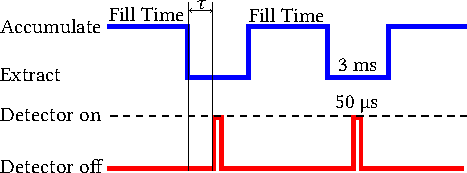
\includegraphics[width = 0.8\textwidth]{main/ShapePulse.pdf}
    \caption{Illustration of the experimental sequence for measuring the temporal shape of ion bunches leaving the first octopole (figure not to scale). Ions are accumulated (blue) over a preset time (data for 500ms, 30sec, and 1 minute were recorded) and then released. The measurement (red) is turned on for 50$\mu$s with a delay $\tau$ with respect to the release of the ions.
    Measurements are repeated 20 times for each value of $\tau$ in order to ensure good statistics. By varying $\tau$ and recording the number of ions a temporal shape of the ion bunch is recorded}
    \label{fig:sequenceShape}
\end{figure}

Results from the measurements when the octopole is allowed to accumulate ions for 500ms, 30 seconds and 1 minute can be seen on 
\cref{fig:bunchShape}. Here three loading times are compared, namely 500ms (green), 30 seconds (blue), and 1 minute (orange).
It is seen that the curves for 30 seconds and 1 minute are highly similar, this is likely because they contain very similar amounts of ions as can be seen in \textcolor{red}{CITE LOADING}.

The 500ms curve however is considerably slower, both in its rise time and its tail, by approximately a factor of 2. This indicates that the number of ions seems to affect the temperature, with fewer ions leading to colder temperatures.
Indeed if we, naively, take the factor 2 difference in time constant to mean that the ions are half as slow, we find that if the ions are loaded for 500ms, they are about a quarter 
of the temperature of the ions that are loaded over 1 minute or 30 seconds.
\begin{figure}[h]
    \centering
    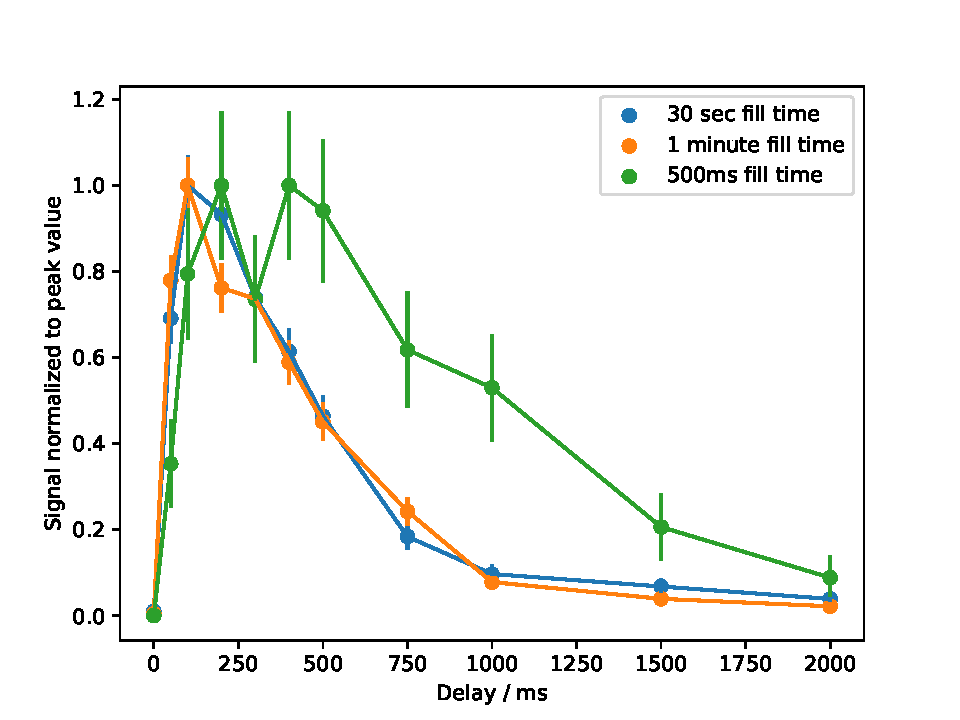
\includegraphics[width = 0.9\textwidth]{main/chargeShape.pdf}
    \caption{Plot showing the temporal shape of ion bunches, when the octopole is allowed to fill for 500ms (green), 30 seconds (blue), and 1 minute (orange).
    Each curve has been normalized to its peak value, in order to allow comparison of the curves. From the measurements it is clear that the majority of ions will arrive during the first second if there are few ions in the octopole (500ms).
    The width of the pulse is shortened considerably down to approx 500ms if the octopole is allowed to fill. Thus if one wants to be careful of saturating the channeltron detector it is likely best to assume that when an ion bunch is released, all the ions will arrive during 500ms, as this allows some overhead.
    A feature to note is that the 500ms curve, seems to have a slope that is approx half as steep as the other two curves at the earliest part of the bunch.
    If one considers the tail we also see that the 500ms curve is approximately a factor two slower here as well. This gives a qualitative indication that loading fewer ions into the octopole, gives a colder distribution of ions}
    \label{fig:bunchShape}
\end{figure}

It is not surprising to see that a higher number of ions in the octopole lead to higher temperatures. Firstly, the octopole is an RF device, and thus there will always be micromotion,
 (much like the quadrupole of \cref{chap:LinTrap}) for any ions that do not lie exactly on the center axis of the octopole. 
As more and more ions are loaded into the octopole, more of them will find their equilibria further off-axis, where the micromotion is larger, leading to hotter ions.

In addition as the number of ions in the storage device increases, ion-ion collisions become more likely. It is known that such collisions in RF devices will lead to heating of the ion cloud \cite{BlumelHeating,MichaelIonIonHeating}.


\subsection{Measuring the fill time of the octopole}
Another characterization that has been performed of the first octopole of the setup is testing how long it takes the octopole to reach the limit of the number of ions it can hold.
In order to test this, the octopole is allowed to fill for a variable time $\tau$, after which the ions are released, and the channeltron detector records the total number of ions.
By doing this for increasing times we expect to see a behaviour where the number of ions increases linearly in time initially, until eventually space charge effects start to play a role.
When these effects come into the picture the loading of ions will progress slower as new ions arriving become able to knock "old" ions out of the octopole, until eventually a steady state is realized.
An illustration of the experimental sequence can be seen on \textcolor{red}{ADD FIGURE}. 


All measurements for this experiment were taken at an ion current of approx 300 ions/second, measured at the channeltron detector.
The ion current measured at the detector usually varies within 10\% due to fluctuations in flow from the electrospray. Thus, any measurements of how long it takes to fill the octopole have to be adjusted for the ion flux during the loading phase.  This adjustment is done by multiplying the physical loading time by the ratio between the reference of 300 ions/s and the mean of the measured current before and after the experiment giving
\begin{equation}
    \tau'= \frac{I_{reference}}{I_{measured}}\tau,\quad I_{measured} = \frac{I_{before}+I_{after}}{2}.
\end{equation}
An illustration of the experimental sequence may be seen on 